\begin{frame}{Events grouped by longTracks vs DeltaR0 }
    \begin{figure}
        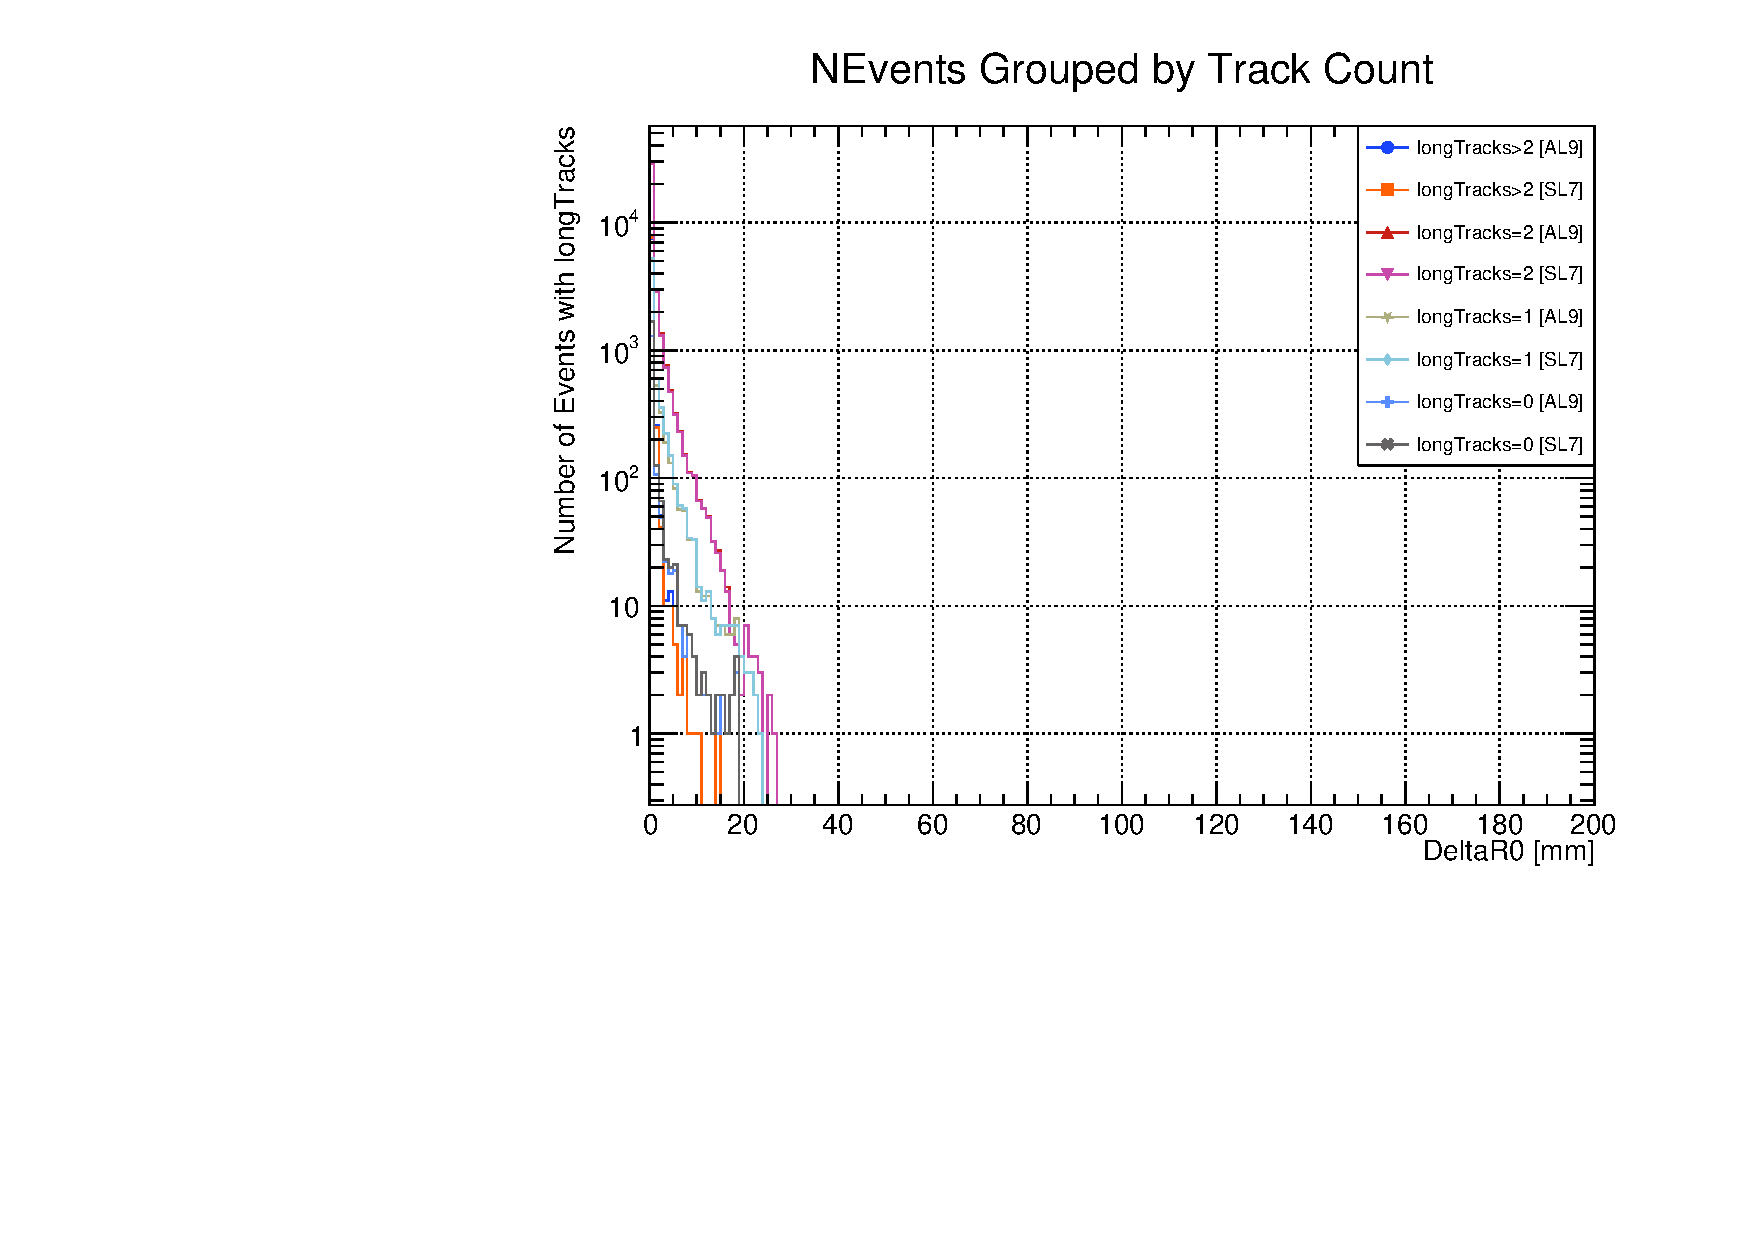
\includegraphics[width=\linewidth]{./output/DeltaR0_all.pdf}
    \end{figure}
\end{frame}

\begin{frame}{Events grouped by longTracks vs DeltaY0 [SKIP]}
    \begin{figure}
        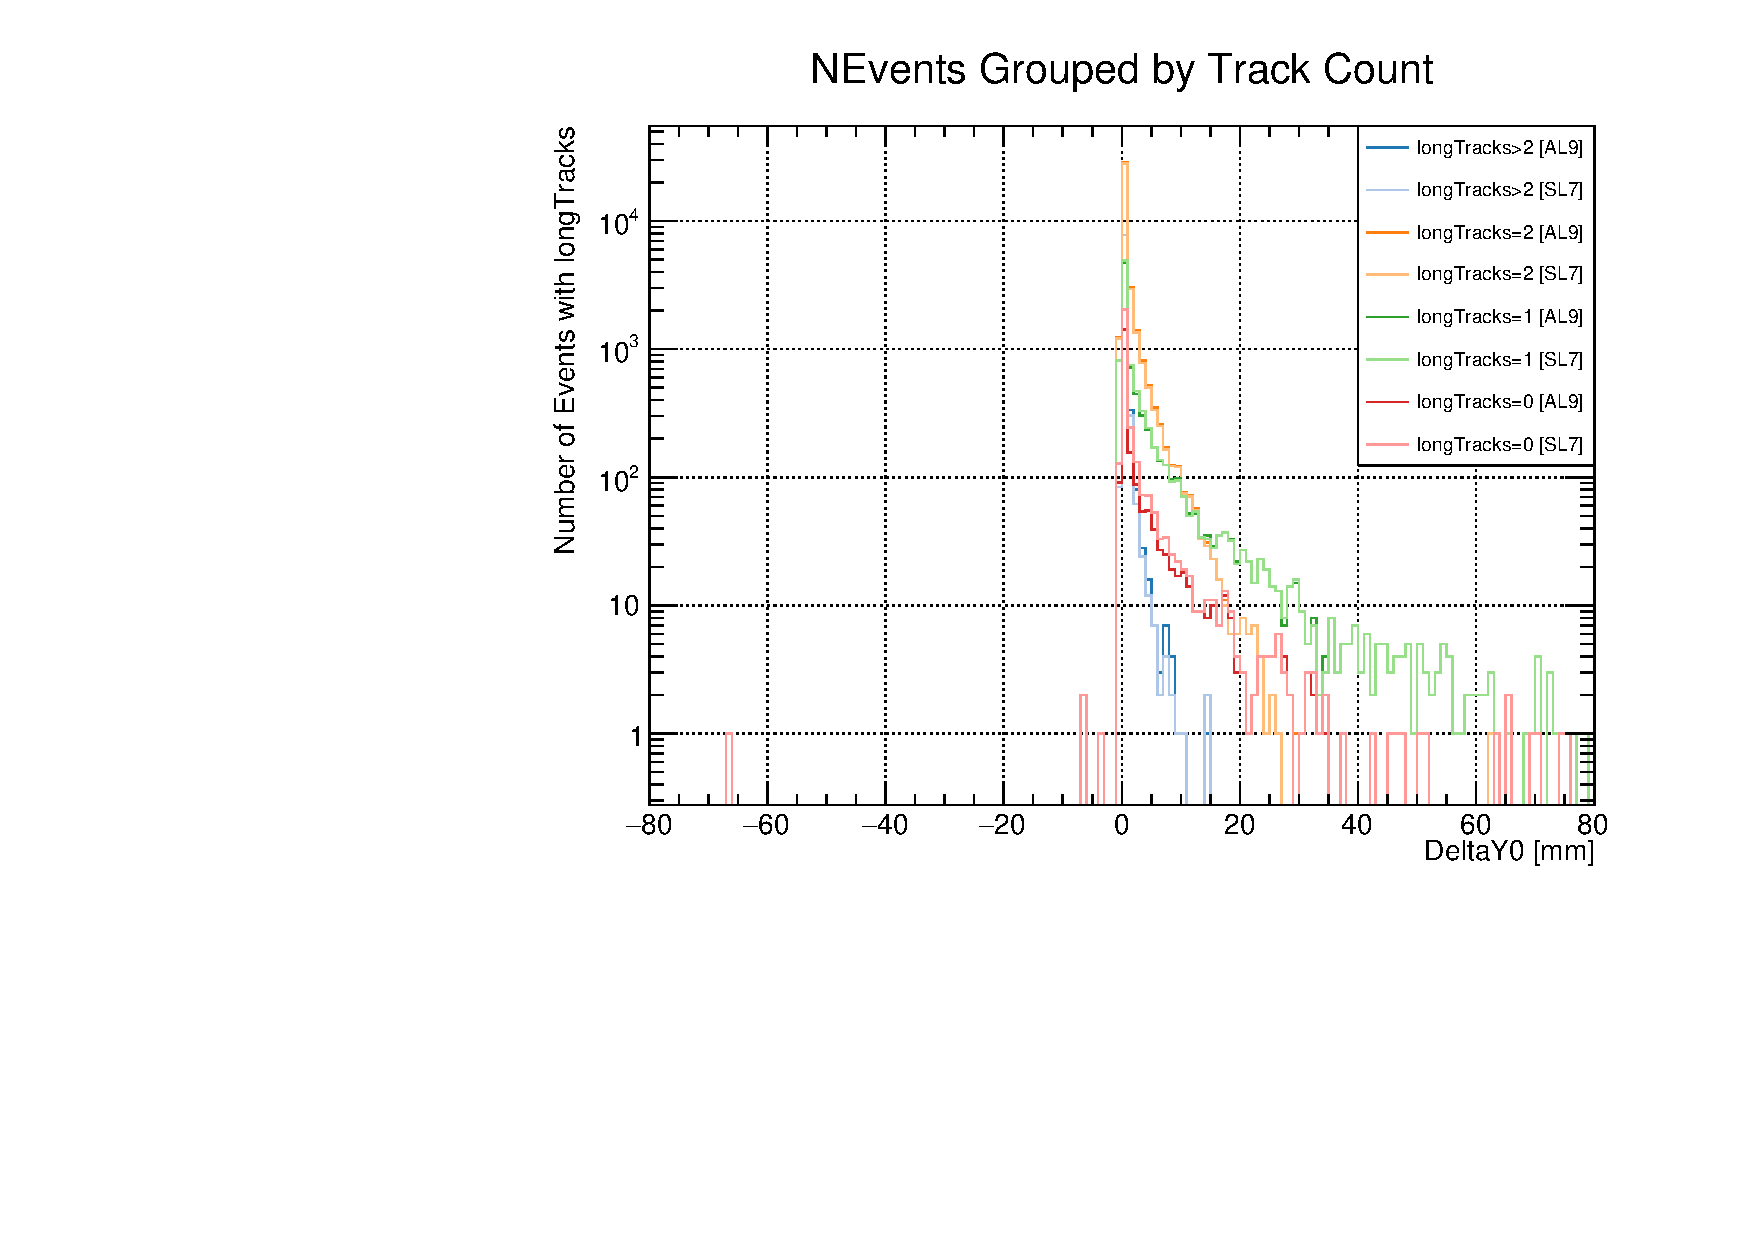
\includegraphics[width=\linewidth]{./output/DeltaY0_all.pdf}
    \end{figure}
\end{frame}

\begin{frame}{Events grouped by longTracks vs DeltaX0 [SKIP]}
    \begin{figure}
        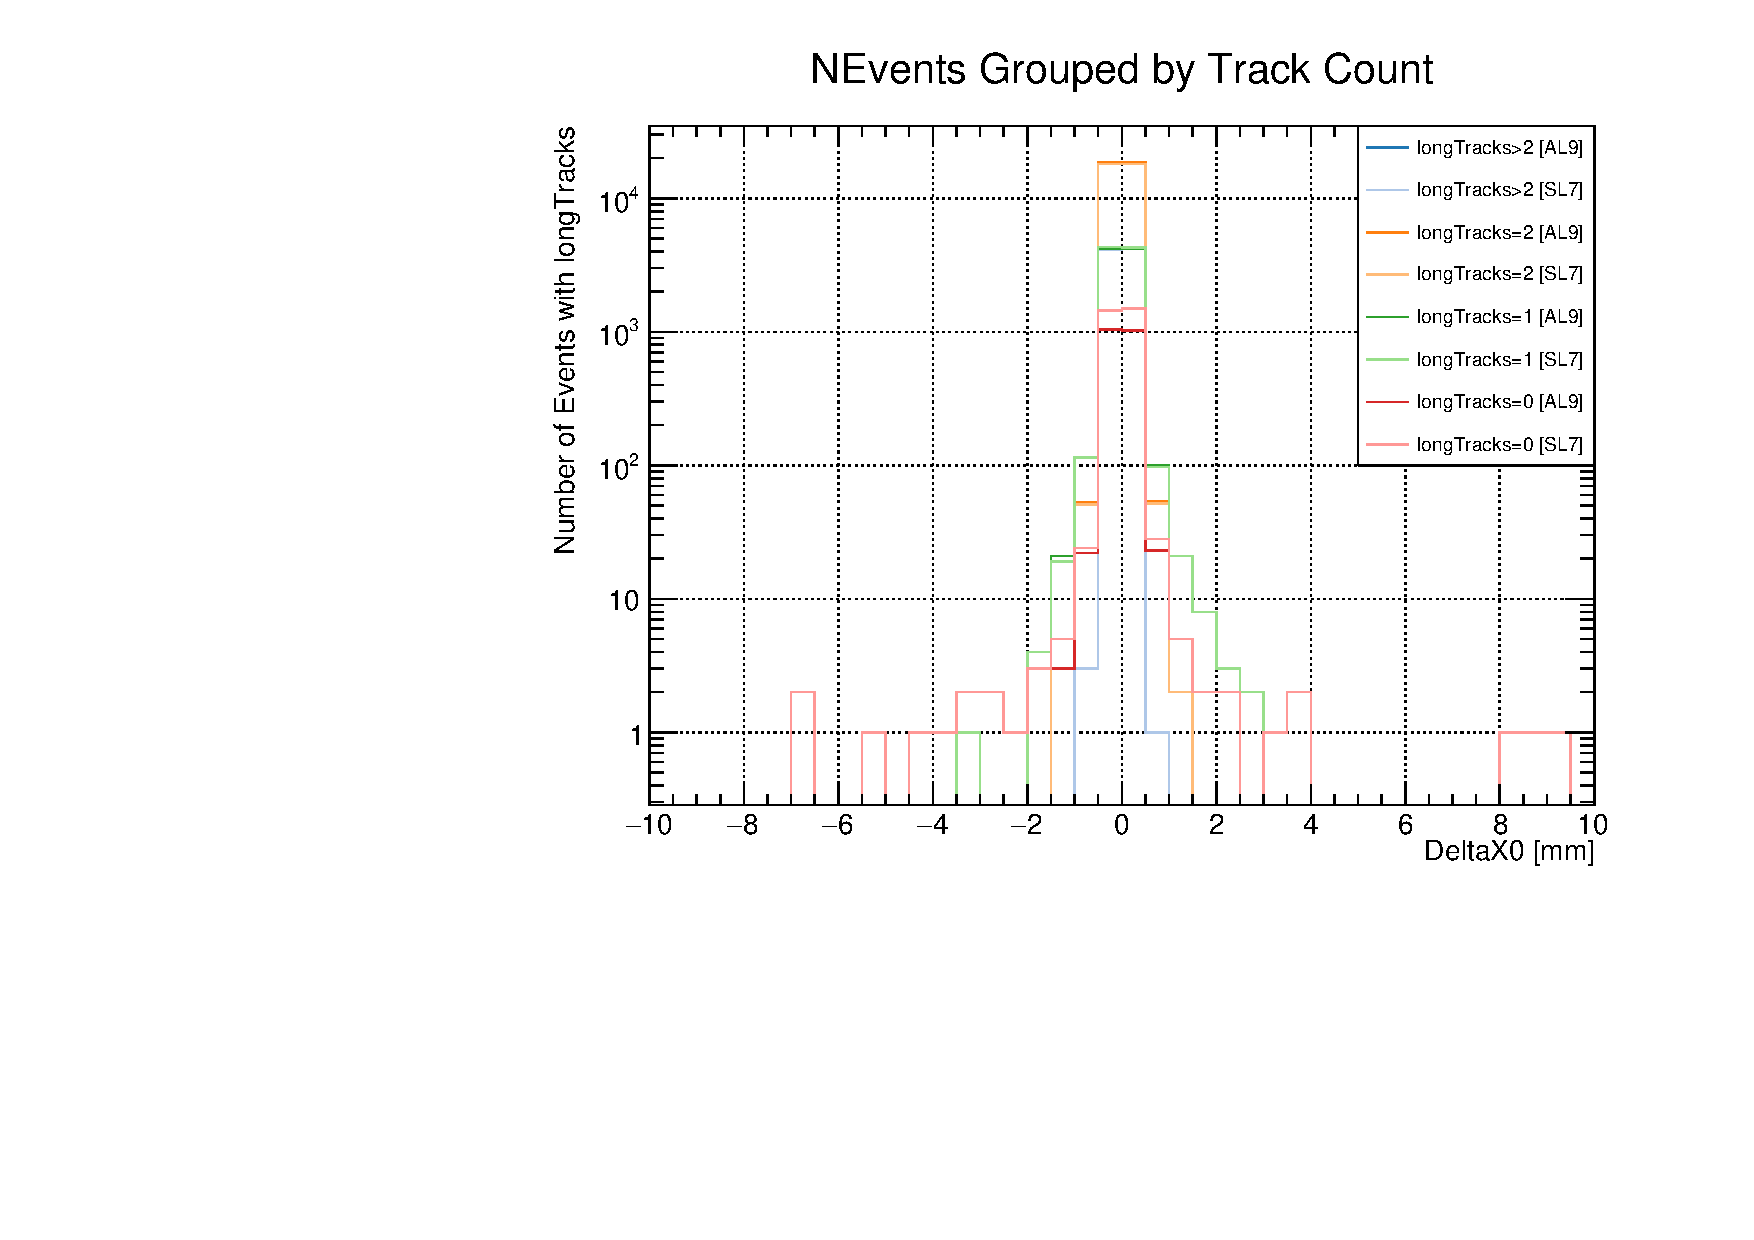
\includegraphics[width=\linewidth]{./output/DeltaX0_all.pdf}
    \end{figure}
\end{frame}

\begin{frame}{Events grouped by longTracks vs Theta0 }
    \begin{figure}
        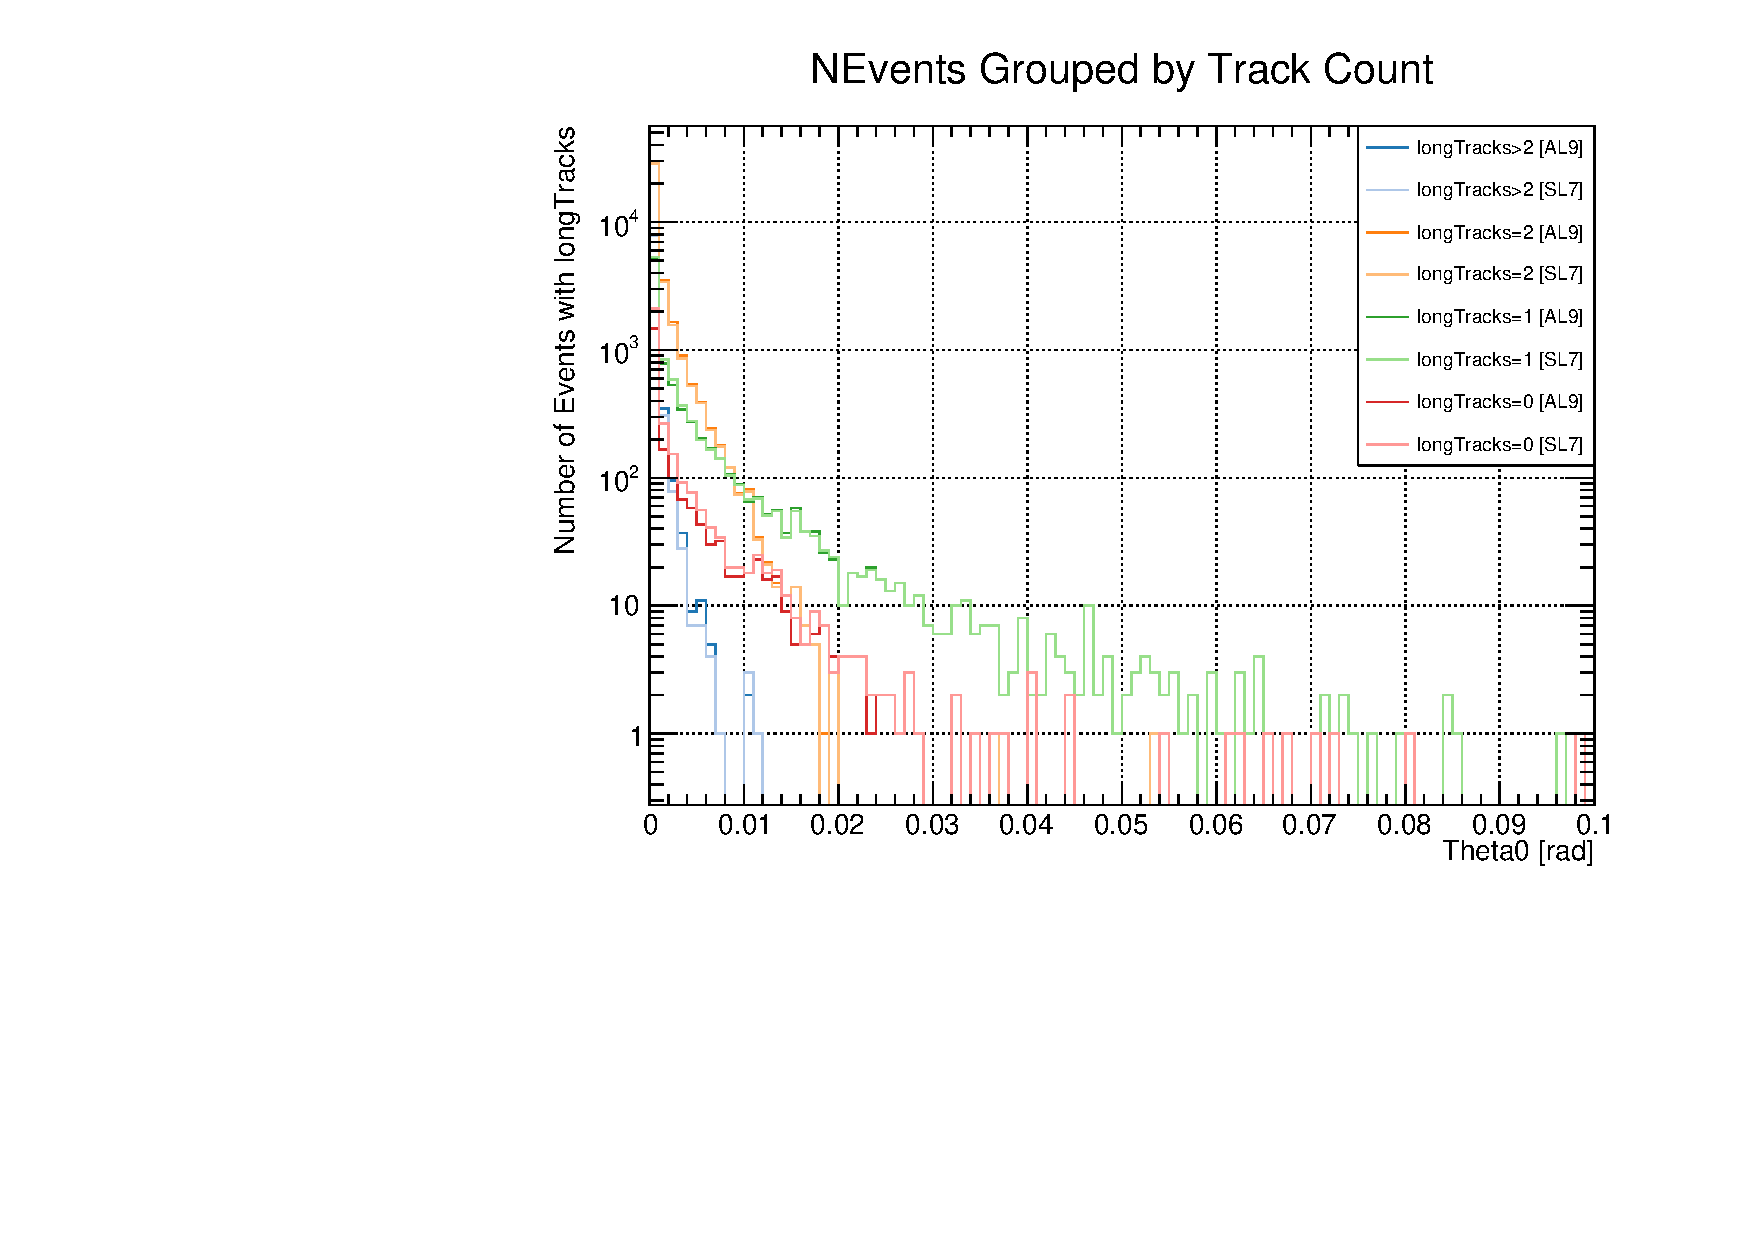
\includegraphics[width=\linewidth]{./output/Theta0_all.pdf}
    \end{figure}
\end{frame}

% \begin{frame}{Two Track Reconstruction Efficiency }
%     \begin{figure}
%         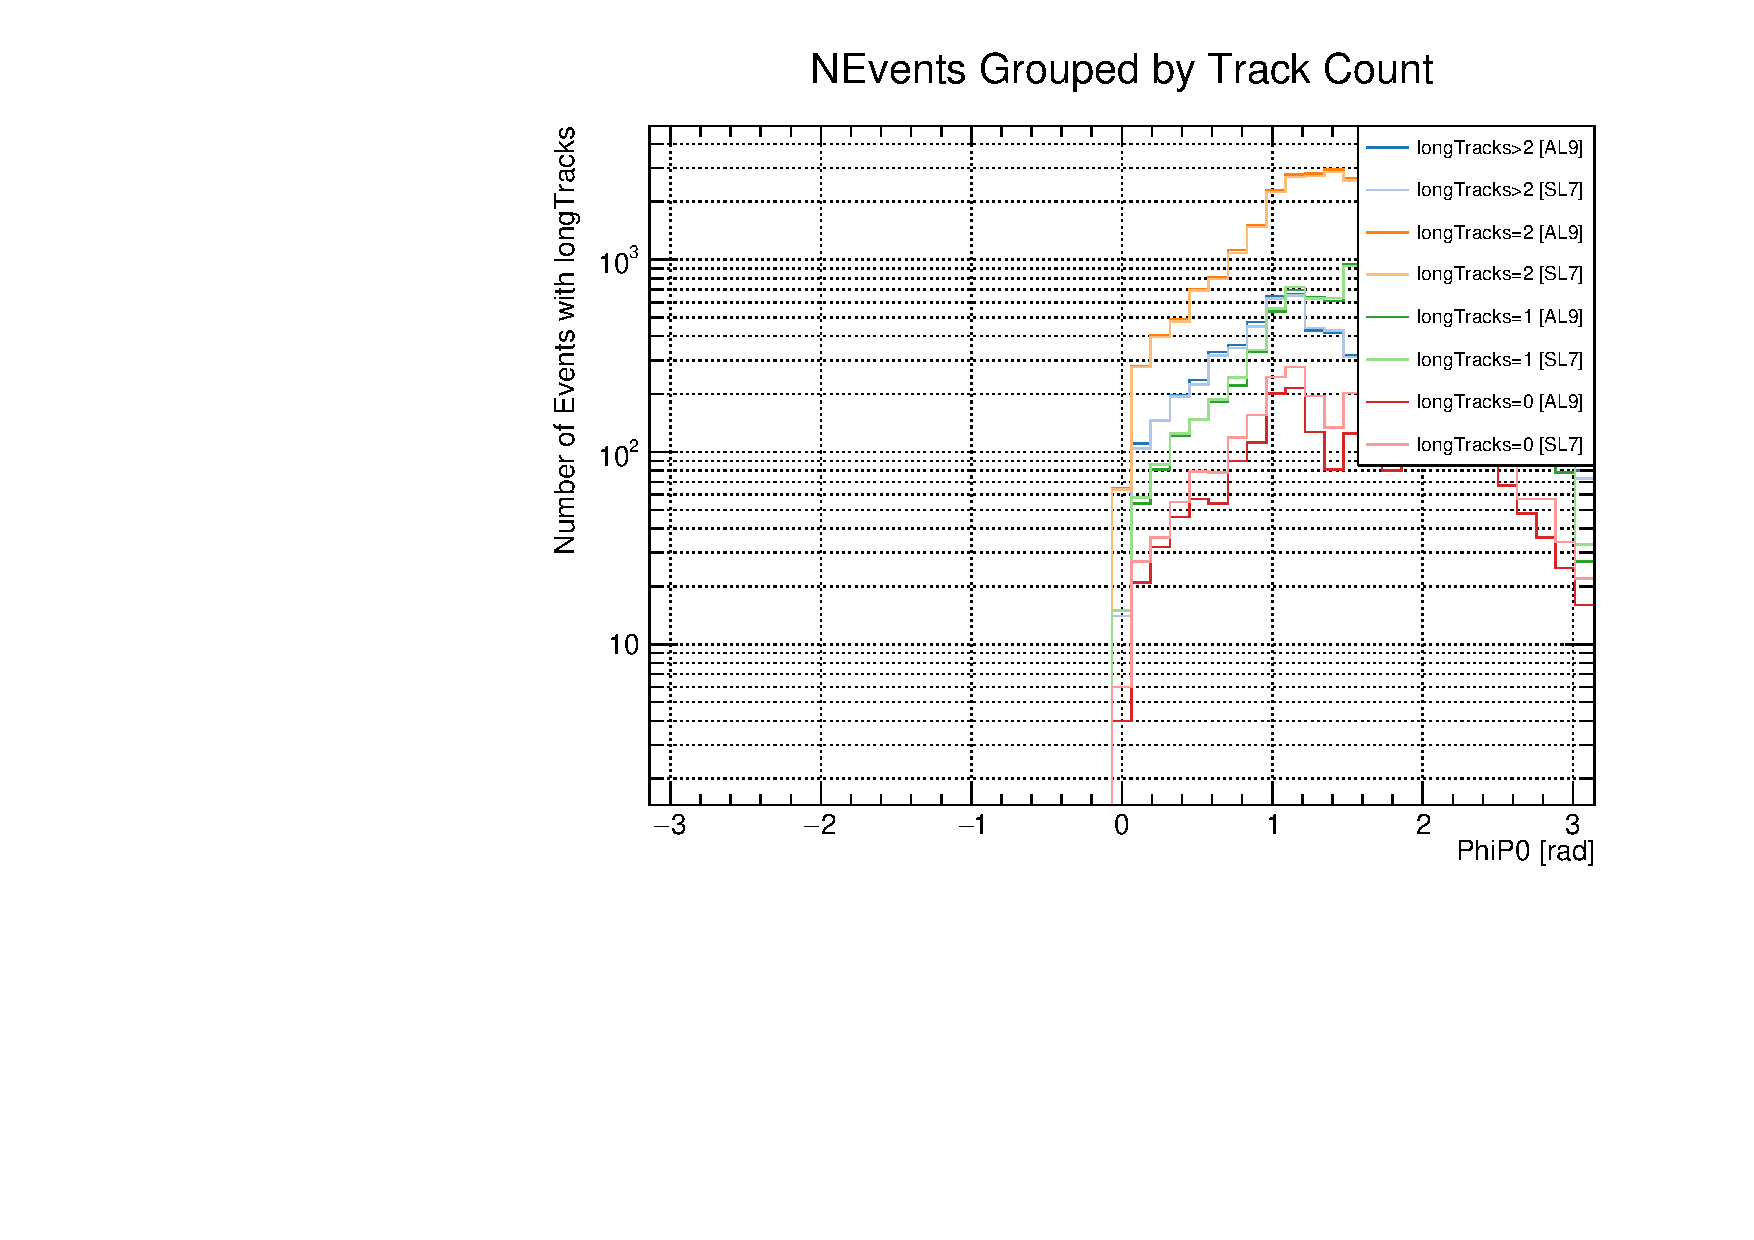
\includegraphics[width=\linewidth]{./output/Effi_PhiP0_all.pdf}
%     \end{figure}
% \end{frame}

\begin{frame}{Events grouped by longTracks vs DeltaRP}
    \begin{figure}
        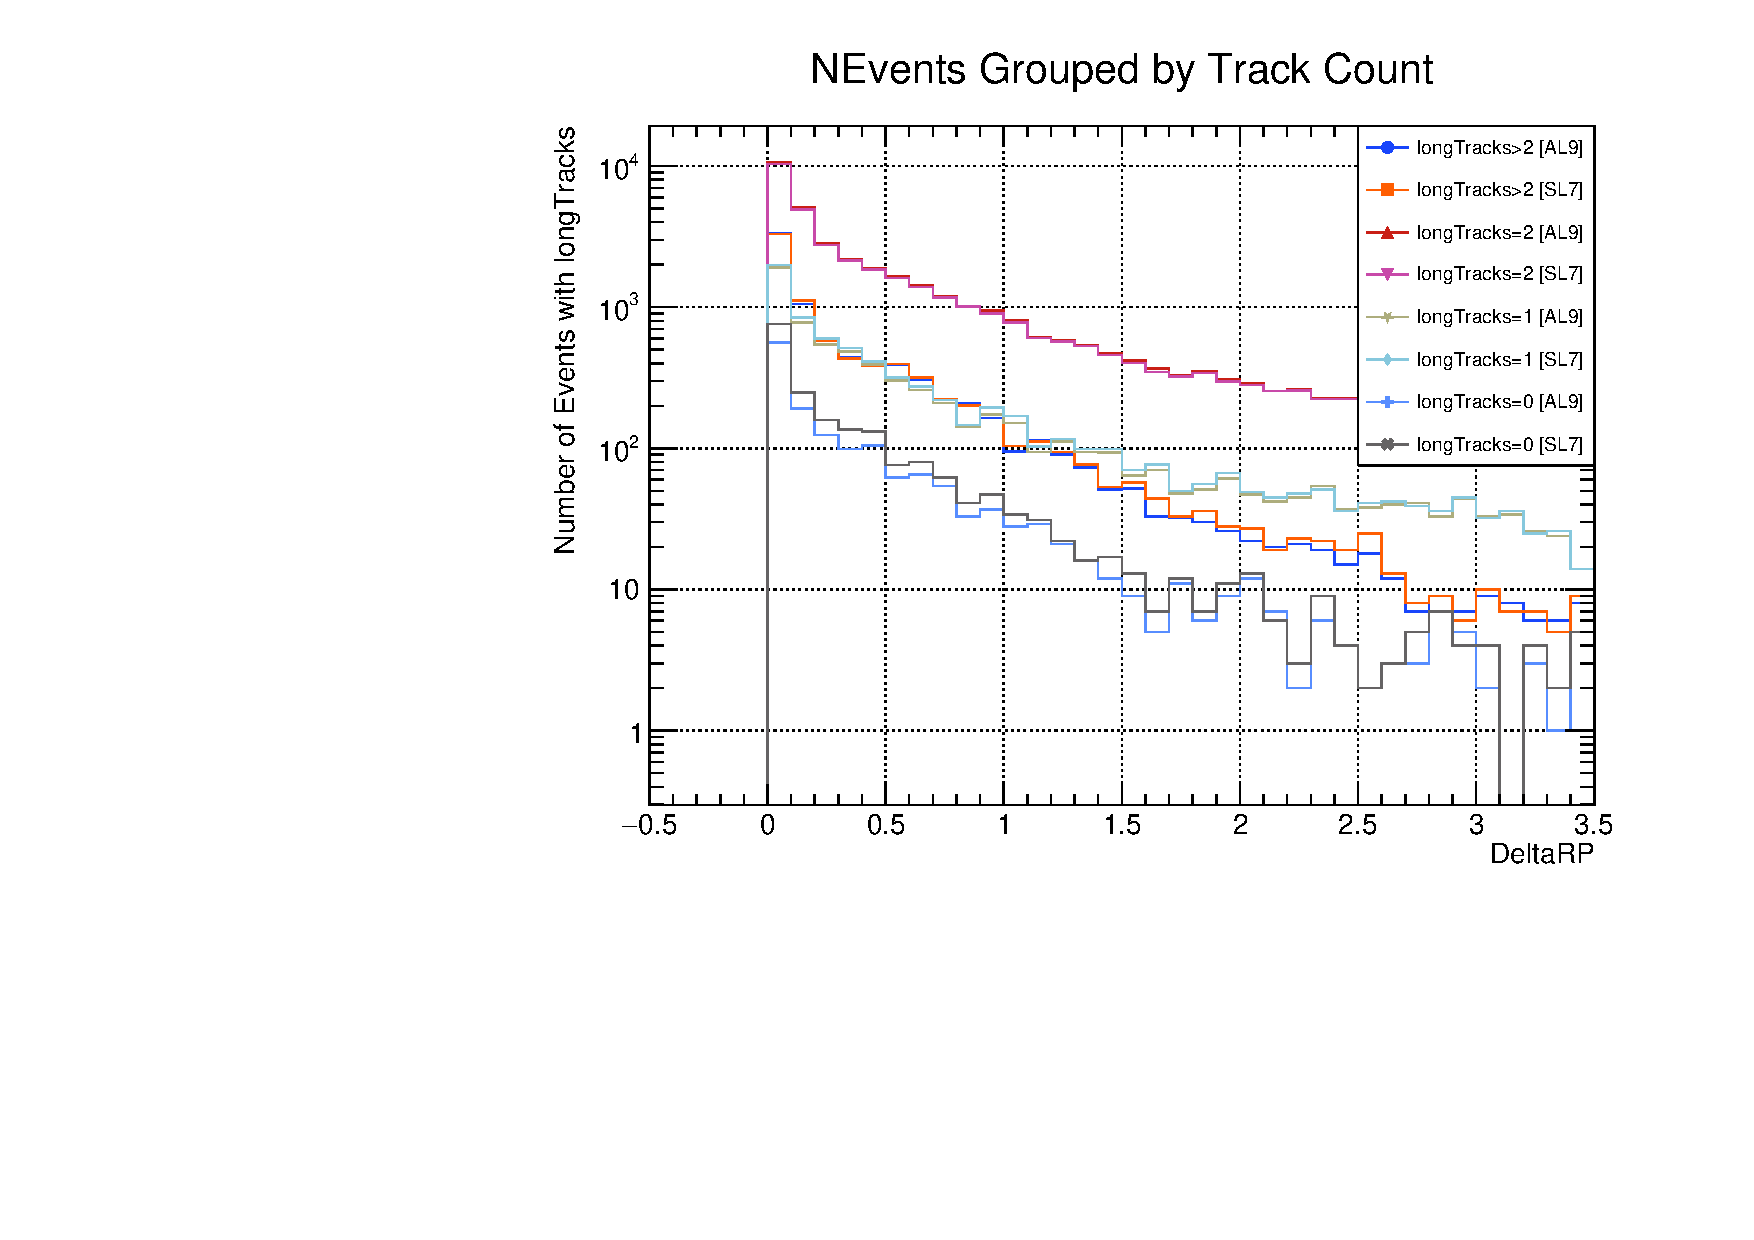
\includegraphics[width=\linewidth]{./output/DeltaRP_all.pdf}
    \end{figure}
\end{frame}

\begin{frame}{Comments on longTrack grouped Plots}
    \begin{itemize}
        \item Good agreement between ALMA9 and CENTOS7
        \item Events with $>2$ longTrack fall most rapidly [nothing past 10 mm]
        \item $=2$ longTracks decay less rapidly [nothing past 30 mm]
        \item $=1$ longTracks is relatively flat
        \item $=0$ same as above - Not sure how to interpret
        \item In the plots where longTracks $\leq$ 1 AL9 performs bad at low separation 
        \item Maybe logscale in x?
    \end{itemize}
    
\end{frame}